\documentclass[a4paper,11pt]{report}
%\usepackage[none]{hyphenat}

%\usepackage[T1]{fontenc}
%\usepackage[bitstream-charter]{mathdesign}

%\usepackage[usenames,dvipsnames,pdf]{pstricks}
%\usepackage[crop=off]{auto-pst-pdf}
\usepackage{makeidx}
\usepackage{url}
\usepackage[square,sort,comma,numbers]{natbib}
\usepackage{framed}
\usepackage[toc,page]{appendix}
\usepackage{graphicx}
\usepackage{longtable}
\usepackage{subfig}
\usepackage{amsfonts}
\usepackage{amsmath}
\usepackage{amsthm}
\usepackage{amssymb}
\usepackage{listings}
\usepackage{tikz}
\usepackage{tcolorbox}
\usepackage{float}
\usepackage{multirow}
%indicator 1
\usepackage{bbm}

% Fancy letters
\usepackage{mathrsfs}

% Fancy lists
%\usepackage{enumerate}  


\usepackage[noend,ruled,noline,linesnumbered,algochapter]{algorithm2e}
\usepackage[linktoc=page]{hyperref}
\usepackage[margin=3cm]{geometry}
\usepackage{setspace} 

\usepackage{fancyhdr}

% add todo package
\usepackage[colorinlistoftodos]{todonotes}

%add hyperref package
\usepackage{hyperref}

%
\usepackage{tikz, tikz-cd}

\pagestyle{fancy}

\rhead{\nouppercase\leftmark}
\lhead{\nouppercase\rightmark}

\makeindex

\onehalfspacing 

\renewcommand*\contentsname{Table of Contents}

% Proof, Corollary, and Lemma indexing
\newtheorem{theorem}{Theorem}[section]
\newtheorem{corollary}{Corollary}[section]
\newtheorem{lemma}[theorem]{Lemma}
\newtheorem*{remark}{Remark}
\newtheorem{example}{Example}[chapter]
\theoremstyle{definition}
\newtheorem{definition}{Definition}[section]
\newtheorem{conjecture}{Conjecture}

% New Commands 
\newcommand{\thm}[2]{\begin{theorem}[#1] #2 \end{theorem} }
\newcommand{\prf}[1]{\begin{proof} #1 \end{proof}}
\newcommand{\eq}[1]{\begin{equation*} #1\end{equation*}}
\newcommand{\eqq}[1]{\begin{equation} #1\end{equation}}
\newcommand{\lem}[1]{\begin{lemma} #1 \end{lemma}}

\newcommand{\CC}{\mathbb C}
% Fancy C
\newcommand{\CE}{\mathcal C}
\newcommand{\FF}{\mathbb F}
% Special F_p 
\newcommand{\FP}{\mathbb{ F}_q}
\newcommand{\KK}{\mathbb K}
% Fancy L
\newcommand{\LL}{\mathcal L}

\newcommand{\NN}{\mathbb N}
% indicatior 1
\newcommand{\OO}{\mathbbm 1}
%Fancy P
\newcommand{\PP}{\mathcal P}
\newcommand{\QQ}{\mathbb Q}
\newcommand{\RR}{\mathbb R}
\newcommand{\SP}{\mathbb S}

% Fancy S
\newcommand{\ES}{\mathcal S}
\newcommand{\ZZ}{\mathbb Z}

%indicator 
\newcommand{\1}[1]{\mathds{1}_{[#1]}}

\newcommand{\sgn}{\text{sgn }}


% headheight to make the problems shut up for once.
\setlength{\headheight}{13.6pt}
\addtolength{\topmargin}{-1.6pt}

\begin{document}

\pagenumbering{roman}

%title page
\begin{titlepage}


    \begin{center}
    \line(1,0){430}\\
    \vspace{5pt}
    %{ \Huge \bf Heuristically Guided\\ Local Search for \\ Protein Structure Prediction \\}
    {\Huge \bf On Polynomial Methods in \\ \vspace{5pt} Combinatorics}
    \line(1,0){430}
    
    \end{center}
    
    \vfill
    
    \begin{center}

    \end{center}
    
    \vfill
    \begin{center}
    {\large \bf  Conrad Crowley }\\
    { \large \bf 118316041}\\
    
    
    \end{center}

    \begin{center}
        {\large \bf  Supervisor: Dr. Marco Vitturi }\\
        { \large \bf Second Reader: Dr. Andrei Mustata}\\
        
        \end{center}
    
    
    \vfill
    
    
    \begin{center}
    \end{center}
    
    \vfill
    \begin{center}
    {Final Year Project 2022}
    \end{center}
    
    \vfill
        
    \begin{center}
    
\includegraphics[scale=0.2]{./images/ucc}
    \end{center}
    
    
    
    \end{titlepage}
    

%\clearpage
%\thispagestyle{empty}
%\mbox{}
\clearpage

%\thispagestyle{empty}
%Dedication
%I would like to dedicate this thesis to my loving family ...
    



%\clearpage
%\thispagestyle{empty}
%\mbox{}
%\clearpage
%\thispagestyle{empty}
\pagenumbering{roman}
\setcounter{page}{1}

%\input{0.1.abstract.tex}

\clearpage
\phantomsection
\tableofcontents
\renewcommand{\contentsname}{Table of Contents}
\addcontentsline{toc}{chapter}{Table of Contents}

\clearpage
\phantomsection
\addcontentsline{toc}{chapter}{List of Figures}
\listoffigures

%\clearpage
%\phantomsection
%\addcontentsline{toc}{chapter}{List of Tables}
%\listoftables



\clearpage
\pagenumbering{arabic}
\setcounter{page}{1}

\renewcommand\bibname{References}

\clearpage
\phantomsection


\chapter{Introduction}
The following is a short exposition of polynomial methods in combinatorics. Polynomial methods are a collection of techniques which use polynomial interpolation and rigidity properties
of polynomials to control the size of collections of objects with a certain structure. 
The first example of this technique was presented in the 1990s in \cite{alon1999combinatorial},  which we examine in detail
in Chapter \ref{chap:alon}. The modern conception of the polynomial method was pioneered by Dvir in 2008 (See \cite{2008DVIR}), where he produced a remarkably short resolution to the finite field analogue of the Kakeya Conjecture which provided
a new framework and enthusiasm for the polynomial method in combinatorial problems. We will explore this proof in the next chapter. 

The most striking feature of the following proofs is that they leverage certain properties of polynomials in problems which on the surface appear not to have anything to 
do with polynomials. Generally, extremal configurations of these problems tend to admit a lot of algebraic structure and this is exactly what these methods exploit using polynomials. 


\section{Why Polynomials?}
It is perhaps wise to discuss here what features of polynomials make them particularly powerful when dealing with problems in Combinatorics. 
Polynomials are perhaps some of the simplest of mathematical objects, as once we define a field they are simply a combination of the addition and multiplication operation between elements. 
It is not immediately obvious why such simple objects may prove to be so useful.

There are two key properties of polynomials that this collection of methods exploit.
Firstly, we use the fact that there are roughly $\sim D^n$ coefficients of a polynomial in $n$ variables of degree at most $D$ (See Lemma \ref{lem:paramcounting}).  This is utilised 
in an essential manner when we try to find polynomials that contain objects in their zero set. We can contain a set of size $M$ in the zero set of
a polynomial with degree at most $O(M^{1/n}$). In other words, we have a lot of flexibility in choosing a polynomial.
Secondly, and in sharp contrast, polynomials behave extremely rigidly when restricted to lines. We mean by this that the zero set of a polynomial of degree $D$ can intersect 
a line in at most $D$ points if the line is not contained within said zero set. The gap between this flexibility of choosing a polynomial and rigidity of restricting to lines provides
us with a surprisingly powerful technique. 

Another striking thing about the method is the non-constructive manner in which the polynomials are usually used. 
We often cannot explicitly find a satisfactory polynomial to use for our purposes, instead we opt to use arguments from Linear Algebra to establish the
existence of a polynomial with such properties. This is reminiscent of other methods in combinatorics, such as the Probabilistic Method or the Topological Method (See \cite{ALON2003} for a survey of these methods). 

\section{Notation}
We introduce some convenient notation here. We write that $A \lesssim_n B$ to mean that there exists some constant
$C(n)$ which depends on $n$ such that $A \leq C(n) B$. Further, we write that $A \sim_n B$ if $A \lesssim_n B$ and $B \lesssim_n A$.

We write $\text{Poly}_D (\KK^n)$ to represent the space of polynomials in $n$ variables with coefficients in a field $\KK$ and degree at most $D$.

The indicator function $\OO$ is defined on logical statements $X$ as follows:
\[
    \OO[X] = 
  \begin{cases}
      1 & \text{if X is true}, \\
      0 & \text{if X is false}.
  \end{cases}  
\]
For any function $f : \RR^n \to \RR$ let us denote the zero set of $f$ by $Z(f) = \{x \in \RR^n \ | \ f(x) = 0\}.$
We borrow from Computer Science the big O notation. For functions $f,g : \NN^+ \to \RR$ we write:
\begin{align*}
    f(N) &= O(g(N)) \iff \exists N_0, M \in \NN \text{ such that } f(n) \leq Mg(n) \forall n > N_0 \\
    f(N) &= \Omega(g(n)) \iff g(N) = O(f(N)).
\end{align*}
These can be thought of as asymptotic upper and lower bounds respectively.
\chapter{The Kakeya Problem in Finite Fields \label{chap:kakeya}}
Before we can discuss the Kakeya problem in finite fields, and its rather surprising resolution, we ought to first discuss the origin and history of the problem. 
Work on the Kakeya problem can be traced back to the Russian mathematician Abram Besicovitch in 1917. While working on a problem in Riemann integration, Besicovitch was led to consider the question of the existence of planar sets of measure zero which contain a line segment in every direction. In 1920, Besicovitch constructed such a set and published in a Russian Journal.

However, 1917 was a turbulent year as it marked the end of
the Russian Empire and the start of the Russian civil war. Due to this and the ensuing blockade of Russian ports there was scarce communication with the outside world.
Thus Besicovitch could not have known of a Japanese mathematician Kakeya who asked also in 1917 a related question: What is the smallest area of a convex set within which
one can rotate a needle by 180 degrees in the plane? Julius Pal answered this question in 1921 with the equilateral triangle in \cite{pal1920elementares}. The 
more interesting problem obtained by dropping the convexity condition remained open. In 1924, after leaving the newly formed Soviet Union for Copenhagen, Besicovitch discovered this
problem and by modifying his previous construction produced a solution in 1925. This lead to the more general questions being asked about Kakeya sets in higher dimensions.
\begin{definition}[Kakeya Set in $\RR^n$]
    A \textbf{Kakeya set} is a set $A \subset \RR^n$ that contains a unit segment in every direction.
\end{definition}
Besicovitch's construction showed that these sets can have arbitrarily small measures, even attaining zero, in $\RR^2$. Further, a straightforward process allows to extend the construction of these measure-zero sets to the case of arbitrary dimension.

Given that Kakeya sets can have measure zero, the natural question then arises, are Kakeya sets fractal in nature? This leads one to consider the dimension of Kakeya sets as a quantification of their fractal nature. There are many notions of dimensions that can be investigated, but we restrict ourselves to the Minkowski and Hausdorff dimensions.

\begin{definition}[Minkowski Dimension]
Given a set $S \subset \RR^n$, define $N(\varepsilon)$ to be the number of cubes of side length $\varepsilon$ required to cover the set.
The \textbf{Minkowski Dimension} of the set $S$ is then defined as
$$\dim_M (S) = \lim_{\varepsilon \to 0} \frac{\log( N(\varepsilon))}{\log (1/\varepsilon)}.$$
If this limit does not exist, one can still define the upper and lower Minkowski dimensions, 
$\dim_{M_{\text{upper}}}$ and $\dim_{M_{\text{lower}}}$, by taking the limit superior and limit inferior respectively.
\end{definition}
\begin{definition}[Hausdorff Dimension]
    We define the $d$-dimensional Hausdorff measure of a set $S \subset \RR^n$ as
    $$\mathcal{H}^d(S)=\lim_{r \to 0} \inf \left\{\sum_i r_i^d:\text{ there is a countable cover of } S\text{ by balls with radii } 0 < r_i < r\right\}.$$
    Then we can define the \textbf{Hausdorff dimension} of the set $S$ to be
    $$\dim_H (S) = \inf \{ d \geq 0 : \mathcal{H}^d(S) = 0 \}.   $$
\end{definition}
These dimensions are related by the following inequality when they are all defined:
$$\dim_H \leq \dim_{M_{\text{lower}}} \leq \dim_{M_{\text{upper}}}.$$
In 1971, Davies published \cite{davies1971some} showing that
although the measure of a Kakeya set in $\RR^2$ can be arbitrarily small, it must have Hausdorff and Minkowski dimension of 2.
This resulted in the following conjectures:
\begin{conjecture}[Kakeya Conjecture for the Minkowski Dimension]
    Let $A$ be a Kakeya set in $\RR^n$. Then $\dim_M (A) = n$. \label{conj:mink-kakeya}
\end{conjecture}
\begin{conjecture}[Kakeya Conjecture for the Hausdorff Dimension]
    Let $A$ be a Kakeya set in $\RR^n$. Then $\dim_H (A) = n$. \label{conj:haus-kakeya}
\end{conjecture}
In a survey on the problem, (see \cite{wolff1999recent}) Wolff proposed a finite analogue to the Kakeya Conjecture. We begin with some preliminaries so we can formally state this analogue.

\begin{definition}[Finite Field]
    A \textbf{finite field} $\FP$ is a field of finite cardinality. 
    The cardinality $|\FP| = q$ of a finite field is called the \textbf{order} of the finite field.
\end{definition}
It is known that finite field of order $q$ exists if and only if $q = p^k$ for some prime $p$ and integer $k$. For the rest of this chapter we let $q$ be of this form.

\begin{lemma}
    Each element $X$ in a finite field $\FF$ satisfies the identity:
    $$X^{|\FF|} - X =0$$
    identically in $\FF$. \label{lem:finite-fields-poly-identity}
\end{lemma}
\begin{proof}
    This lemma follows immediately from Fermat's Little Theorem.
\end{proof}


A Kakeya set in $\FP^n$ is a set that contains a line in every direction. In analogy to the Euclidean case, we formally define lines in $\FP^n$ as the sets of the form
$$\ell_{x,y} = \{x+ty :  t \in \FP \}$$
for some fixed $x,y \in \FP^n$ with $y\neq 0$.
It should be noted that a line in a finite field $\FP^n$ contains exactly $|\FP|$ points.
Formally, directions in $\FP^n$ can be identified using the projective space $\mathbb{P}\FP^n  = \FP^n/\FP^\times$. In this projective space, two lines $y$ and $y'$ are equivalent if $y'$ is a translation of $y$.
The finite analogue to Conjectures \ref{conj:mink-kakeya} and \ref{conj:haus-kakeya} is:
\begin{conjecture}[Kakeya Conjecture in Finite Fields]
    If $A\subset \FP^n$ contains a line in every direction, then $|A| \gtrsim_n |\FP|^n $. \label{KakeyaConjecture}
\end{conjecture}
This conjecture had a significant influence on the subject, inspiring work on the sum-product phenomenon in finite fields. From its postulation in 1999,
little progress was made in the following years and it was assumed that the problem was roughly as difficult as the Euclidean case. 

In 2008, Dvir published a remarkably simple proof of Conjecture \ref{KakeyaConjecture} using elementary facts about polynomials (See \cite{2008DVIR}). 
This proof revitalised interest in the polynomial method, and we shall explore its details later in this chapter. 

\begin{figure}[h]
\centering 
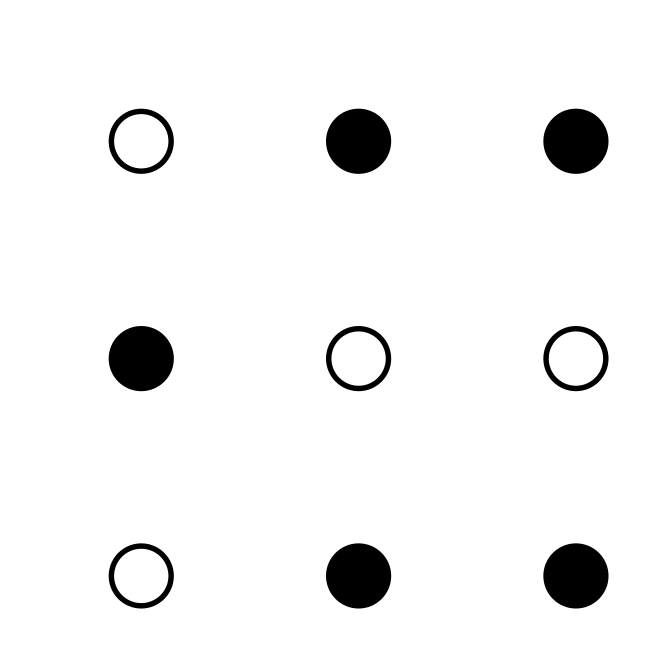
\includegraphics[width=0.3\textwidth]{images/kakeya_ex_f32.png}}
\caption{An example of a Kakeya set (shaded) in $\FF_3^2$.}
{\label{kak_ex_f32}
\end{figure}






\section{Combinatorial Attempts}
To truly show the power of the polynomial method, we shall first explore purely combinatorial attempts 
at estimating the sizes of Kakeya sets. All the following estimates are much weaker than the bound in Theorem \ref{KakeyaConjecture}.
We fix a finite field $\FF = \FF_{p^k}$ where $p$ is a prime. 

Our first estimate shows that Conjecture \ref{KakeyaConjecture} is true for the $n$ = 2 case.

\begin{lemma}
    Suppose $s \leq |\FF|$. If $l_1, \dots, l_s$ are distinct lines in $\FF^n$, then their union has cardinality at least $(1/2)|\FF|s$. \label{lem:kak-first-estimate}

    In particular, if $A \subset \FF^n$ is a Kakeya set, then we have
    \[
      |A| \gtrsim |\FF|^2.
    \] 
\end{lemma} 
\begin{proof}
    We add the lines together one at a time and track the cardinality of their union. The first line contains $|\FF|$ points. The second line must contain at least $|\FF| -1$ points not in the first line. Similarly the third line must contain at least $|\FF| -2$ points not in the first two lines, and so on. Thus the number of distinct points in the union of all $s$ lines is given by
    \[
      \sum_{i=1}^{s} |\FF| - i + 1  > (1/2) |\FF| s.
    \]

    A Kakeya set always contains at least $|\FF|$ lines, so setting $s=|\FF|$ above yields
    \[
        |A| > (1/2) |\FF|^2 .
    \]

\end{proof}

\subsection{Bush Argument} 
Bourgain produced one of the first non-trivial estimates of the dimension in his work \cite{BUSH1991}. We present the finite field analogue of his argument here (See \cite{GUTH2016}). This argument is known as the ``bush'' argument as we consider a high-multiplicity point through which pass many lines, forming a ``bush'' around that point. 


\begin{theorem}[Bush Argument]
If $A \subset \FF^n$ is a Kakeya set, then we have
$$|A| \gtrsim |\FF|^{\frac{n+1}{2}}.$$
\end{theorem}

\begin{proof}
    Let $\mu$ be a fixed multiplicity parameter to be chosen later. Either there exists a point $p\in A$ such that there are $\mu$ lines passing through $p$,
    or else every point in $A$ has less than $\mu$ lines passing through it.

    In the first case, since the lines have distinct directions they must become disjoint when $p$ is removed. Hence
    \[
      |A| \gtrsim \mu |\FF| .
    \]

    In the latter case, by double counting we have
    \begin{align*}
         \sum_{\ell \subset A} \sum_{p \in A} \OO[p \in \ell] &= \sum_{\ell \subset A} |\FF| = |\FF|^{n-1} |\FF| \\
        \sum_{p \in A} \sum_{\ell \subset A} \OO[p \in \ell] &\leq \sum_{p \in A} \mu = |A|\mu \\
        \implies \frac{|\FF|^{n}}{\mu} \leq |A|.
    \end{align*}
    Now we optimise the two lower bounds by choosing $\mu \sim |\FF|^{\frac{n-1}{2}}$, so that in either of the above cases we obtain
    \[
        |A| \gtrsim |\FF||\FF|^{\frac{n-1}{2}} \sim |\FF|^{\frac{n+1}{2}}.
    \]

\end{proof}

\subsection{Hairbrush Argument}
In \cite{WOLFF1995}, Wolff presented the ``hairbrush'' argument where he made an incremental improvement over the argument of Bourgain. It is similar in spirit to the ``bush'' argument above, 
however instead of using just one point of high-multiplicity we instead consider a line (or ``stem'') containing many points of high-multiplicity.

\begin{theorem}[Hair Brush Argument]
    If $A \subset \FF^n$ is a Kakeya set, then we have
    \[
        |A| \gtrsim |\FF|^{\frac{n+2}{2}}.
    \]
\end{theorem}
\begin{proof}
Let $\mu$ be a fixed multiplicity parameter to be chosen later. We say a line $\ell$ is $\mu$-rich if for at least $|\FF|/2$ points $p\in \ell$ there are $\mu$ lines distinct from $\ell$
in $A$ passing through $p$. Either there exists a $\mu$-rich line or there does not. 

Suppose a $\mu$-rich line exists, and denote this line by $\ell_\mu$. Consider the family $\Pi$ of 2-dimensional planes passing through $\ell_\mu$. 
If a line $\ell$ intersects $\ell_\mu$ then there exists a unique plane $\pi \in \Pi$ such that $\ell, \ell_\mu \in \pi$. 
Let $\LL_\pi := \{\ell \subset \pi \ | \ \ell \cap \ell_\mu \neq \emptyset \}$. The set $A \cap \pi$ is a set in (an isomorphic copy of) $\FF^2$ that contains at least $|\LL_\pi|$
lines, and hence by Lemma \ref{lem:kak-first-estimate} we have
\[
|A \cap \pi| \gtrsim |\LL_\pi| |\FF|.
\]
Thus,
\[
    |A| \geq \sum_{\pi \in \Pi} |(A \cap \pi) \backslash \ell_\mu| \gtrsim |\FF| \sum_{\pi \in \Pi} |\LL_\pi| \gtrsim \mu |\FF|^2,
\]
where the last inequality comes from the fact $\ell_\mu$ intersects at least $\mu |\FF|/2$ lines, so since the planes $\Pi$ foliate $\FF^n$, the union $\cup_\Pi \LL_\pi$ contains at least all of these lines.

Suppose there does not exist a $\mu$-rich line. Let 
\[
    A' = \{p \in A \ | \ p \text{ belongs to strictly less than } \mu \text{ lines in }A \}.
\]
Since we assume there does not exist a $\mu$-rich line in $A$, for any line $\ell \subset A$ we have $|A' \cap \ell| > |F|/2$. 
Proceeding by double counting, 
\begin{align*}
    |A| &\geq |A'|\geq \frac{1}{\mu} \sum_{p \in A'} \sum_{\ell \subset A} \OO[p \in \ell] \\
    &= \frac{1}{\mu} \sum_{\ell \subset A} |A' \cap \ell| \gtrsim \frac{1}{\mu} |\FF|^{n-1}|\FF|\\
    \implies |A| &\gtrsim \frac{|\FF|^n}{\mu}.
\end{align*}
Now optimising the two lower bounds by choosing $\mu \sim |\FF|^{\frac{n-2}{2}}$, so that in either of the above cases we obtain the bound
\[
    |A| \gtrsim |\FF|^2|\FF|^{\frac{n-2}{2}} \sim |\FF|^{\frac{n+2}{2}}.
\]
\end{proof}

\section{Dvir's Proof \label{sect:Dvirs-proof}}
Again we fix $\FF = \FF_{p^{q}}$ for some prime $p$.
\begin{theorem}[Kakeya Conjecture in Finite Fields]
    If $A\subset \FF^n$ contains a line in every direction, then $|A| \geq \frac{1}{n!} |\FF|^n $. \label{thm:Kakeya}
\end{theorem}
We shall prove this theorem via three surprisingly elementary lemmas. The general strategy of the proof is to assume the size of a Kakeya set $A$ is small and find a low-degree non-zero polynomial that interpolates (contains in its zero set) the points in $A$. We then show that due to the structure of the Kakeya set the polynomial's zero set must contain many more points. This contradicts the fact our polynomial is non-zero and of low-degree which  establishes the Kakeya Conjecture over finite fields.


The first lemma is a fundamental one to the polynomial method, exploiting the flexible interpolation properties of polynomials. 
Consider the problem of finding a non-zero polynomial in $\RR[X,Y,Z]$ of the minimal possible degree that vanishes at the points $(j,k, 2^{j^k})$ for $1\leq i \leq 10^{6}$. 
If we try to find an explicit polynomial we may produce
\begin{align*}
    P(X,Y,Z) &= \prod_{j,k=1}^{10^{6}} (X-j) (Y-k) 
    \intertext{or perhaps}
    Q(X,Y,Z) &= \prod_{j,k=1}^{10^{6}} (Z-2^{j^k}).
\end{align*}
Both $P$ and $Q$ vanish on our points and it is difficult to explicitly produce a polynomial of much lower degree that also satisfies this property.
One might consider taking the product of linear factors in $\RR[X,Y,Z]$, constructing the polynomial to vanish on sets of planes defined by three points in the collection.
Such a polynomial has a degree of $\lceil \frac{1}{3} 10^{12}\rceil $, which is slight improvement on 
$Q$ which has a degree of $10^{12}$. Naively one might conjecture that the degree of any polynomial with this property is of the order of $10^{12}$. 
Remarkably, the following lemma shows that we can find such a polynomial with a degree of about $\sim 18000$. This polynomial has roughly $\sim 18000^3$ coefficients and as such the polynomial is quite difficult to explicitly write, but we can establish the existence of such a polynomial non-constructively.
\begin{lemma}[Parameter Counting] 
Let $\KK$ be a (not necessarily finite) field. If $A \subset \KK^n$ and $|A| < {{n+D} \choose {n}}$, there exists a non-zero polynomial $P(X_1,\dots, X_n)$ of degree at most $D$ that vanishes on $A$. \label{lem:paramcounting}
\end{lemma}

\prf{ We first show the dimension of $\text{Poly}_D (\KK^n)$ is ${D+n} \choose{n}$. A basis for $\text{Poly}_D (\KK^n)$ is given by monomials of the form $X_1^{D_1}\dots X_n^{D_n}$, where $\sum_i D_i \leq D$, hence we just need to count the number of monomials.

We can map a monomial $X_1^{D_1}\dots X_n^{D_n}$ to a string of $D$ $\star$'s and $n$ $|$'s as follows. 
Begin with $D_1$ $\star$'s, then place one $|$. We put now $D_2$ $\star$'s, and place a second $|$. 
We continue until we have placed $D_n$ $\star$'s followed by an $n^{\text{th}}$ $|$. 
Finally we place $D - \sum_i D_i \star$'s.
 This is a bijective map between the monomials in $\text{Poly}_D (\KK^n)$ and all the strings of $D$ $\star$'s and $n$ $|$'s. 
 To assemble such a string we distribute the $n$ $|$'s over $n+D$ spaces, and then fill the remainder with $\star$'s. Hence we get the binomial coefficient
$$\text{Poly}_D (\KK^n) = {{n+D} \choose{n}}.$$

Now let $p_1, \dots, p_{|A|}$ be the points of $A$. We consider the evaluation map $E: \text{Poly}_D (\KK^n) \to \KK^{|A|}$ defined by
$$E(Q) = \left(Q(p_1), \dots, Q(p_{|A|})\right).$$

This map is clearly linear. 
Its kernel $\ker E$ is exactly the set of polynomials in $\text{Poly}_D (\KK^n)$ that vanish on $A$. 
By assumption, the dimension of $\text{Poly}_D (\KK^n)$ is greater than $A$, so the dimension of the domain of $E$ is greater than the codomain of $E$. By the rank-nullity theorem, we conclude $E$ must have a non-trivial kernel. 
Thus there exists a non-zero polynomial $P \in \text{Poly}_D (\KK^n)$ that vanishes on $A$.} 


Note that if $D=|\FF|-1$, and $|A| \leq {{|\FF|+n-1} \choose{|\FF|-1}} = { {|\FF|+n-1} \choose{n}}$ we have a polynomial of degree at most $|\FF|-1$ that vanishes on $A$. 
Since $\frac{|\FF|^n}{n!} < {{|\FF|+n-1} \choose{n}}$, we can certainly find such a polynomial when $|A| \leq \frac{|\FF|^n}{n!}$. The restriction of $D=|\FF|-1$ is somewhat necessary due to the fact that polynomials with a factor of $X^{|\FF|} - X$ vanish identically by Lemma \ref{lem:finite-fields-poly-identity}.



\begin{lemma}Suppose $A \subset \FF^n$ contains a line in every direction, and suppose that there exists a non-zero polynomial $P$ with degree $D<|\FF|$ that vanishes on $A$. Then there exists a non-zero degree $D$ polynomial $\bar{P}$ that vanishes everywhere on $\FF^n$. \label{lem:kaklem2} \end{lemma}

\prf{ Choose a line in $A$, say $\ell = \{x+ty : t\in \FF \}$ with $x,y\in \FF^n$ and $y \neq 0$. Now we consider the restriction of our polynomial $P$ to the line $\ell$, $P_{|\ell}$.
Recall $P$ is a sum of monomials, and we use multi-index notation here with $\alpha = (\alpha_1, \alpha_2, \dots, \alpha_n), \ \alpha_i \in \NN \cup \{0\}$ and $|\alpha| =  \sum \alpha_i$. $P$ can be written as
$$P(X_1,X_2, \dots, X_n) = \sum_{|\alpha| \leq D} c_{\alpha} X_1^{\alpha_1}X_2^{\alpha_2}\dots X_n^{\alpha_n}. $$
Now $P_{|\ell}$ can be written
$$P_{|\ell} = P(x+ty) = Q_{x,y}(t) = \sum_{|\alpha| \leq D} c_\alpha \prod_{i} (x_i + t y_i)^{\alpha_i}.$$
We now wish to examine the degree $D$ term of $Q$,
which consist in the terms of the expansion of the expression above obtained by the product of the $ty_i$ terms when $|\alpha| = D$. 
 
This is related to the degree $D$ component $Q_D$ of $Q$ by the identity
$$Q_{x,y,D} = t^D Q_D(y) = t^D \sum_{|\alpha| = D} c_\alpha \prod_i y_i^{\alpha_i}.$$

Now if $P_{|\ell}$ vanishes everywhere on $\ell$, since its dependence on $t$ is given by a polynomial of degree less than $|\FF|$, all its coefficients must be zero. In particular, we must have $Q_{x,y,D} = 0$.
This is clear from the factor theorem, as we could write the roots of $P_{|\ell}$ as $(t-k_1)(t-k_2)\dots(t-k_{|\FF|})$; but this contradicts the fact $P$ is of degree $D < |\FF|$.

Notice that $Q_{x,y,D}$ no longer depends on $x$, but on $y$ alone. In particular $Q_D(y) = 0$, but $y$ was an arbitrary non-zero element of $\FF^n$, and $Q_D(y)$ also vanishes at zero, so it vanishes everywhere. Thus we can pick $\bar{P}$ = $Q_D$, and we are done.
}

Finally, we show that any non-zero polynomial in $\FF[X_1, \dots, X_n]$ with degree less than $|\FF|$ cannot be zero everywhere in $\FF^n$.

\lem{Let $P$ be a non-zero polynomial on $\FF^n$ with degree less than $|\FF|$. Then $P$ does not vanish everywhere. \label{lem:kaklem3}}

\prf{ We proceed by induction on $n$. For $n=1$, a non-zero polynomial that vanishes everywhere has $|\FF|$ roots, so must be at least of degree $|\FF|$.
Let us assume that the statement holds in $\FF^{n-1}$, we now prove it must also hold for $\FF^n$.

We proceed by contradiction, assuming that $P$ vanishes everywhere. We let $X_1, \dots ,X_n$ be coordinates on $\FF^n$, and we write $P$ in the form

$$P(X_1, \dots ,X_n) = \sum_{j=n}^{|\FF|-1} P_j(X_1, \dots X_{n-1}) X_n^j.$$

Each $P_j$ are polynomials in $X_1, \dots X_{n-1}$ of degree less than $|\FF|$. Fix $X_1, \dots X_{n-1}$, and let $X_n$ vary. Now we have a polynomial in $X_n$ of degree less than $|\FF|$ that vanishes for all $X_n \in \FF$. By the base case this must be the zero polynomial. So each $P_j(x_1, \dots, x_{n-1}) = 0$ for all $j$ and for all $(x_1, \dots x_{n-1}) \in \FF^{n-1}$. Now by induction on $n$, each $P_j$ is the zero polynomial. Then $P$ is the zero polynomial as well. 
}
We now combine these lemmas to establish the Kakeya conjecture over finite fields.
\begin{proof} [Proof of Theorem \ref{thm:Kakeya}] 
Assume $A \subset \FF^n$ is a Kakeya set, and that $|A| \leq \frac{|\FF|^n}{n!}$. Then by Lemma \ref{lem:paramcounting} we can find a 
non-zero polynomial of degree at most $|\FF|-1$, say $P$, that vanishes on $A$. Now by Lemma \ref{lem:kaklem2} there exists a non-zero polynomial $\bar{P}$ that vanishes everywhere on $\FF^n$, and has degree less than $|\FF|$.
Finally, Lemma \ref{lem:kaklem3} says that such a $\bar{P}$ is necessarily the zero polynomial, a contradiction. We conclude that $|A| > \frac{|\FF|^n}{n!}$, or in other words
$$
|A| \gtrsim_n |\FF|^n.
$$
\end{proof}

\begin{remark}
    Theorem \ref{thm:Kakeya} lends a good degree of support for Conjectures \ref{conj:mink-kakeya} and \ref{conj:haus-kakeya} as it essentially rules out purely algebraic counter-examples.
\end{remark}
\chapter{The Polynomial Method in Additive Combinatorics \label{chap:alon}}
So far our discussion has only centred around the usefulness of polynomial methods in combinatorial problems with a geometric flavour. 
In this chapter we shall discuss applications to the exciting field of additive combinatorics, where in 1990 Alon provided perhaps
the first example of the polynomial method in action.\cite{alon1999combinatorial} We present Michalek's short, elementary, and direct proof of the combinatorial nullstellensatz.\cite{michalek2010}
\section{Combinatorial Nullstellensatz}
\begin{theorem}[Combinatorial Nullstellensatz]
    Let $\KK$ be a (not necessarily finite) field, and let $P(X_1,\dots, X_n) \in \KK[X_1,\dots, X_n]$ be a polynomial in $n$ variables with coefficients in $\KK$. Suppose the coefficient of $X_1^{k_1}X_2^{k_2}\dots X_n^{k_n}$ is non-zero and further suppose $\deg P = \sum_{i=1}^n k_i$, where each $k_i$ is a non-negative integer.

    Then for any subsets $A_1,\dots A_n$ of $\KK$ satisfying $|A_i| > k_i$ for each $1\leq i\leq n$ there exist $a_1 \in A_1, \dots, a_n \in A_n$ such that $P(a_1,\dots, a_n) \neq 0$.
    \label{thm:comb-nullstellensatz}
\end{theorem}
\begin{proof}
    We proceed by induction on $\deg P = D$. When $D=1$, $P$ is simply a linear combination of $n$ variables say $P(X_1,\dots X_m) = c_1 X_1 + \dots c_n X_n$. Without loss of generality assume $x_1$ has a non-zero coefficient and consider the sets $A_i = \{a_{i,1}, a_{i,2}\}$. Suppose $P$ at the point $(a_{1,1}, a_{2,1}, \dots, a_{n,1})$ is zero. We can then determine $c_{1} =- \frac{c_2 a_{2,1} + c_3 a_{3,1}+\dots+ c_n a_{n,1}}{a_{1,1}}$. Now evaluating at $(a_{1,2}, a_{2,1}, \dots, a_{n,1})$ we see that this is zero only when $a_{1,1} = a_{1,2}$, so our theorem holds. 

    Now let us assume the theorem holds for $\deg P = D -1$, and prove for $\deg P = D$.
    Suppose that $P$ satisfies the assumptions of the theorem but $P(x) = 0$ for every $x \in A_1 \times \dots \times A_n$.
    Without loss of generality $k_1 > 0.$ Fixing $a\in A_1$ we can write
    \[
    P = (x_1-a)Q +R  \tag{$\dagger$}
    \]
    by the usual long division of polynomials. The degree of $R$ in $x_1$ must be strictly less than $\deg(X_1-a)$, so $R$ is independent of $X_1$ terms. Thus it follows that $Q$ must have a monomial with non-zero coefficient of the form $X_1^{k_{1} -1} X_2^{k_2} \dots X_n^{k_n}$ and 
    $\deg (Q) = D-1$.

    Take any $x \in \{a\} \times A_2 \times \dots \times A_n$ and evaluate $(\dagger)$. Since $P(x) = 0$ it follows that $R(x) = 0$. Hence $R$ vanishes identically on the slice $\{a\} \times A_2 \times \dots \times A_n$. Since $R$ is independent of $X_1$ it must also vanish identically on $A_1 \times A_2 \times \dots \times A_n$.
    Now take any $x \in A_1 \backslash \{a\} \times A_2 \times \dots \times A_n$ and evaluate $(\dagger)$. Since the $(X_1 - a)$ term is non-zero, $Q(x) =0$. So $Q$ vanishes on all $x \in A_1 \backslash \{a\} \times A_2 \times \dots \times A_n$, which contradicts the inductive hypothesis.
\end{proof}
\section{Cauchy-Davenport Theorem}
\begin{theorem} [Cauchy-Davenport Theorem]
    Let $A,B$ be non-empty subsets of $\ZZ_p$ for some $p$ prime. Define their sumset $A+B$ as follows:
    \[
    A + B = 
    \left\{ x \in \ZZ_p\ | \ x = a+b \text{  for some } a\in A, \ b \in B \right\}.
    \]
    Then we have:
    \[
    |A+B| \geq  \min \left\{p, |A| + |B| -1 \right\}.
    \]
\end{theorem} \todo{Generalise this!}

\begin{proof}
    Let us tackle the two cases separately. First, assume that $\min \left\{p, |A| + |B| -1 \right\} = p$.
    Then if $|A| + |B| > p$, $A$ and $B$ must intersect. \todo{expand PHP}
    For some $g \in \ZZ_p$ denote the set  $\left\{ g - x  \ | \ x \in B, \  \right\} \subset \ZZ_p$ as $g-B$. Since $|g-B| = |B|$, we have that 
    $g-B$ and $A$ must intersect as well. Thus there exists some $a \in A$, $b \in B$ such that: 
    \begin{align*}
        g& -b = a \\
        g& = a+b.
    \end{align*}
    Our choice of $g$ was arbitrary, so it follows that $A+B = \ZZ_p$ and hence $|A+B| = p$.

    Now assume that $\min \left\{p, |A| + |B| -1 \right\} = |A| + |B| -1$. Then if the theorem is false we have $|A+B| \leq |A| + |B| -2$, so there exists some $C \subset \ZZ_p$ such that 
    $A+B \subset C$ and $|C| =  |A| + |B| -2$. Now let us define a polynomial $f(x,y) \in \ZZ_p [X,Y$ as:
    \[
        f(X,Y) = \prod_{c \in C} (X+Y -c).
    \]
    Since $A+B \subset C$, $f(a,b) =0$ for all $(a,b) \in A\times B$. Further, the degree of $f$ is $\deg f = |C| = |A| + |B| -2$. 
    We can now appeal to the \hyperref[thm:comb-nullstellensatz]{Combinatorial Nullstellensatz} to yield a contradiction. Let $k_1 = |A| -1$, and $k_2 = |B|-1$. 
    Now $\deg f = k_1 + k_2$, and the coefficient of $x^{k_1}y^{k_2}$ is
    ${|A|+|B| - 2} \choose {|A|- 1}$ which is non-zero in $\ZZ_p$ as the binomial coefficient is not divisible by $p$ if all its factors are less than $p$. Applying Theorem \ref{thm:comb-nullstellensatz} we see that there 
    must exist some $(a,b) \in A \times B$ such that $f(a,b) \neq 0$, a contradiction.
\end{proof}
\chapter{The Joints Problem \label{chap:joints}}
\begin{definition}
    Let $\LL$ be a set of distinct lines in $\RR^n$. A \textbf{joint} of $\LL$ is a point which lies in three non-coplanar lines of $\LL$.
\end{definition}
The joints problem consists in obtaining a sharp upper bound on the maximal number of joints that can be formed from a configuration of $L$ distinct lines.
We denote this quantity $J(L)$. In other words $J(L)$ is the supremum over all configurations of lines in $\RR^n$ of the number of joints.

The joints problem was first posed in 1990 by Chazelle et al in \cite{chazelle1990counting}. They focused on the 3-dimensional case of the problem, establishing a lower bound of $\Omega (N^{3/2})$ and an upper bound estimate of $O(N^{7/4})$. 
This upper bound exponent has fallen gradually throughout the years, the best result prior to the application of the polynomial method being due to Sharir and Feldman in \cite{feldman2005improved} where they established an upper bound of $O(N^{112/69})$. Their
proof uses an array of tools from combinatorial geometry, including forbidden subgraphs in extremal graph theory, space decomposition techniques, and some results from the geometry of lines in space.

\section{Examples}
We shall begin by examining an example based on a grid, in order to gain better intuition about the problem and to formulate a conjecture. 
\begin{example}Consider an $N \times N \times N$ regular grid of integer coordinates in $\RR^3$. We shall give a collection of lines such that each point of this grid is a joint for the collection.
Let $\LL$ be the collection of all lines parallel to any of the Cartesian axes that intersect a point in this grid.
For each horizontal $N \times N$ layer, there are $N+N = 2N$ such lines that intersect our grid. 
There are $N$ layers, so we obtain $2N^2$ distinct lines in this manner. Finally we need to account for the $N^2$ lines perpendicular to the horizontal $N\times N$ layers.
This leaves us with $|\LL| = 3 N^2$ lines forming $N^3$ joints. The number of joints is thus $\sim$ $|\LL|^{3/2}$. 
\end{example}
\begin{figure}[h]
    \centering
\begin{tikzpicture}
    \draw [step=0.5] (0.25,0.25) grid (5.25,4.25);
\end{tikzpicture}
\caption{A $N \times N$ layer of our grid.}
\end{figure}

We can extend this example to higher dimensional grids easily. 
\begin{example}
If we have an $\overbrace{N \times \dots \times N}^{n \text{ Dimensions}}$ regular grid of integer coordinates in $\RR^n$, we can construct an example  by a straightforward extension
of the above example. Each additional dimension increases the number of lines by a factor of $N$ (this can be seen by considering each new dimension as a layering of the previous set along the new axis).
Thus we can see that $\sim N^{n-1}$ lines form $N^n$ joints in this manner. So the number of joints is $\sim |\LL|^{\frac{n}{n-1}}$.
\end{example}

It turns out that the examples illustrated above provide asymptotically maximal configurations, that is, the best configurations disregarding the best constant $C$ such that $J(L) \leq CL^{\frac{n}{n-1}}$.
\section{Solution of the Joints Problem}
This solution was first produced by Guth-Katz for the three-dimensional case in \cite{guth2008algebraic} and later extended to the general case by Quilodrán in \cite{quilodran2009joints} and independently at the same time by 
Kaplan-Sharir-Shustin in \cite{kaplan2009lines}.  


\begin{theorem}
    In $\RR^n$ we have
      $$J(L) \lesssim_n L^{\frac{n}{n-1}}.$$
\end{theorem}
We begin with the fundamental lemma to this proof. The key extension of the polynomial method here over that of Chapter \ref{chap:kakeya} is the examination of directional derivatives of polynomials.
\begin{lemma}
    If $\LL$ is a set of lines in $\RR^n$ that determines $J$ joints, then one of the lines contains at most $nJ^{\frac{1}{n}}$ joints. \label{joints_bound}
\end{lemma}
\begin{proof}
Let $P$ be a non-zero polynomial that vanishes at every joint of $\LL$ and assume that the degree of $P$ is minimal. By parameter counting (Lemma \ref{lem:paramcounting}) the degree of $P$ is at most 
$nJ^{\frac{1}{n}}$. (To see this, set $D = \lfloor nJ^{\frac{1}{n}}\rfloor$ and then notice that $J < {{D+n}\choose {n}}$.)

We proceed by contradiction. Assume every line contains more than $nJ^{\frac{1}{n}}$ joints.
 Now $P$ must vanish on every line in $\LL$ as the degree of $P$ is less than the number of joints contained in the line, which are points of intersection between the line and $Z(P)$.

We now examine the gradient of $P$ at each joint in $\LL$. We will need a fact about gradients for this, which we encapsulate in the following lemma for clarity.
\begin{lemma}
    If $x$ is a joint of $\LL$, and if a smooth function $F: \RR^n \to \RR$ vanishes on the lines of $\LL$, then $\nabla F$ vanishes at $x$. 
\end{lemma}
\begin{proof}
    The joint $x$ is contained in $n$ non-coplanar lines $l_1, \dots, l_n$ with directions $v_1, \dots , v_n$ respectively. 
    Now consider the directional derivative for a particular $v_i$
    \[
    \frac{\partial F}{\partial v_i} (x) = \lim_{t \to 0} \frac{ \overbrace{F(x+ tv_i)}^{F \equiv 0 \text{ on a line in $\LL$}} - \overbrace{F(x)}^{F \equiv 0 \text{ on joints}}}{t} = \frac{0}{t} = 0.    
    \]
    Notice that $ \frac{\partial F}{\partial v_i} = \langle \nabla F, v_i\rangle$ so since we have this for each $v_i$, and the set of $v_i$'s form a basis of $\RR^n$ we have that $\nabla F(x) = 0$.
\end{proof}
So we see that the partial derivatives of $P$ vanish at each joint. The derivatives are polynomials of
smaller degree than $P$ and since $P$ was assumed to be a non-zero polynomial of minimal degree that
vanishes at each joint, each derivative of $P$ must be identically zero. This implies $P$ must be
constant, which is 
a contradiction.
\end{proof}
Finally we can prove the main result. 
\begin{proof}
Lemma \ref{joints_bound} tells us that if we remove a line from our collection, we are removing at most 
$n J(L) ^{\frac{1}{n}}$ joints. By repeating this process, we get the chain of inequalities

\begin{align*}
    J(L) &\leq J(L-1) + n (J(L))^{\frac{1}{n}}\\
    &\leq J(L-2) + 2\left[ n (J(L))^{\frac{1}{n}}\right]\\
    &\leq J(L-3) + 3\left[ n (J(L))^{\frac{1}{n}}\right]\\
&\vdots\\
    &\leq L \left[ n (J(L))^{\frac{1}{n}}\right].
    \intertext{Rearranging we have}
    J(L)^ {\frac{n-1}{n}} &\lesssim_n L \implies J(L) \lesssim_n L ^{\frac{n}{n-1}}.
\end{align*}
\end{proof}


\chapter{Szemerédi-Trotter Theorem \label{chap:trotter}}

In this chapter we will study the application of the polynomial method to incidence geometry by proving a fundamental theorem in the field.
Incidence geometry is the study of possible intersection patterns of simple geometric objects, such as lines or low degree curves. 
We have already seen an incidence problem in the previous chapter on the Joints problem. 
By developing the powerful tool of polynomial partitioning we shall see the key role that the topology of $\RR^n$ can play in such problems, 
in contrast to the trivial topology of finite fields. 


\section{Background}
The Szemerédi-Trotter theorem is a fundamental theorem to the field of incidence geometry, originally proved by an involved cell decomposition argument
of Szemerédi and Trotter and later given a shorter proof using crossing numbers by Székely. 
\begin{theorem}[Szemerédi-Trotter]
    Let $\ES \subset\RR^2$ be a finite set of points and
    let $\LL \subset \RR^2$ be a finite set of lines. We define 
    \[I(\ES,\LL) = \{(p, \ell) \in \ES \times \LL \ | \ p \in \ell\}\] 
    to be the set of incidences between $\ES$ and $\LL$. 
   
    Then:
    \[
        |I(\ES, \LL)| \lesssim \left(|\ES||\LL|\right)^{2/3} + |\ES| + |\LL|
    \]
    \label{thm:S-T}
\end{theorem}

\section{The Trivial Bound}
In planar geometry, we have the following dual statements: two points determine a line and every pair of lines intersect in at most one point.
Using this we can prove the following bounds on $I(\ES,\LL)$:
\begin{theorem}[Trivial Bounds]
    For a set of points $\ES$ and lines $\LL$ we have
    \[I(\ES,\LL)| \leq |\ES|^2 + |\LL|. \]
    \[I(\ES,\LL)| \leq |\LL|^2 + |\ES|. \]
    \label{thm:trivial-ST-bounds}
\end{theorem}
\begin{proof}

To see this, count the lines that have at most one point in $P$ on them. These contribute at most $|\LL|$ incidences.
Every other line has at least two points in $\ES$. The total number of incidences on these lines is at most $|\ES|^2$
as otherwise there would exist a $p\in \ES$ that lies on over $|\ES|$ lines, and each of these lines would have an additional 
point on it. This would imply there are more that $|\ES|$ points, a contradiction. 

Interchanging the roles of $\LL$ and $\ES$ achieves the other bound as two lines intersect in at most one point.
\end{proof}

\begin{theorem}[Second Trivial Incidence Bound]
    $$I(\ES,\LL) \lesssim |\ES|\cdot |\LL|^{\frac{1}{2}} + |\LL|$$
    and
    $$I(\ES,\LL) \lesssim |\LL|\cdot |\ES|^{\frac{1}{2}} + |\ES|.$$
    \label{thm:pretty-trivial-ST-bounds}
\end{theorem}
\begin{proof}
    


We now bound the number of incidences. 

\begin{align*}
    |I(\ES,\LL)|^2 &= \left( \sum_{\ell \in \LL} \sum_{p \in \ES} \OO[p\in \ell] \right)^2 \\
    & \leq |\LL|\cdot \sum_{\ell \in \LL} \left( \sum_{p \in \ES} \OO[p\in \ell] \right)^2  \qquad \text{ (Cauchy-Schwarz on $\ell$)}\\
    &= |\LL|\cdot \sum_{p_1,p_2 \in \ES} \sum_{\ell \in \LL}   \OO[p_1\in \ell] \OO[p_2\in \ell]    \\
    & \leq |\LL|\cdot ( |I(\ES,\LL)| + |\ES|^2)\\ 
    &\leq |\LL|^2 + 2|\LL|\cdot |\ES|^2 \qquad \text{ (Using Theorem \ref{thm:trivial-ST-bounds}) }\\ 
\end{align*}    \todo{extra step needed here - split up sum and do triple thing}
This implies
$$I(\ES,\LL) \lesssim |\ES|\cdot |\LL|^{\frac{1}{2}} + |L|.$$ 
Repeating the above proof interchanging the roles $\ES$ and $\LL$ achieves the other bound.
\end{proof}


\section{Examples}
We can not improve beyond our second trivial bounds in a finite field $\FF^2$. 
\begin{example}[Finite Fields]
Consider the set of points $\ES=\FF^2$ and let $\LL$ be the set of all lines 
in $\FF^2$. Every line contains exactly $|\FF|$ many points of $\ES$, so we have $|\FF|^3$ incidences. 
So both sides of the \hyperref[thm:pretty-trivial-ST-bounds]{second trivial bound} are comparable:
$$
I(\ES,\LL) = |\FF|^3 \sim (|\FF|^2)(|\FF|^2)^{1/2} + |\FF|^2.
$$
\end{example}
In contrast, the following examples seem to be the best possible over $\RR$. We will later prove that these are the asymptotically tight case of the \hyperref[thm:S-T]{Szemerédi–Trotter Theorem}.
We define a line in $\RR^2$ as follows:
\[
    \ell_{m,c} = \{(x,y) \in \RR^2 \ | \ y = mx+c\}.     
\]
\begin{example}
    Consider the following collections in $\RR^2$:
    \begin{align*}
    \ES &= \{ (a,b) \in \ZZ^2 \ | \ a\in [1,N], b \in [1,2N^2] \} \\
    \LL &= \{ \ell_{m,c} \in \RR^2 \ | \ m,c\in \ZZ, m\in [1,N], c \in [1,N^2] \} \end{align*}
    The collection $\ES$ contains $2N^3$ points and $\LL$ contains $N^3$ lines. Every line in $\LL$ contains $N$ points in $\ES$ as for each $x \in [1,N]$  the y-coordinate of $\ell_{m,c}$, $ mx+c$, gives a different integer in $[1,2N^2]$.
    Hence there are $N^4$ incidences. Both sides of the \hyperref[thm:S-T]{Szemerédi-Trotter} inequality are comparable as 
    $$ I(\ES,\LL) = N^4 \sim (N^3)^{\frac{2}{3}} (N^3)^{\frac{2}{3}} \sim |\ES|^{2/3} |\LL|^{2/3}$$
\end{example}
\todo{diagram?}
\begin{example}
    Let $N \gg 1$ be a large even integer and let $1<R \ll N$ be another integer. Consider the collections in $\RR^2$:
    \begin{align*}
        \ES &= \{ (a,b) \in \ZZ^2 \ | \ (a,b) \in [-N/2,N/2] \times [-N/2,N/2] \} \\
        \LL &= \{ \ell \ | \ \ell \text{ contains between R and 2R points of } \ES \} \end{align*}
    We begin by estimating how many lines pass through a given point of the regular grid $\ES$.
    Let $\ell \in \LL$ and $p \in \ES$. The closest point $p' \in \ES$ such that $p \neq p'$ and $p' \in \ell$ must lie
    in a square centred at $p$ of side length $\sim N/R$. This follows from the fact that there are at least $\sim R$ points of $\ES$ in $\ell$ and hence the
    projections of these points to the axes can be separated by at most $\sim N/R$. Taking each possible combination of these we can conclude that there are $\lesssim N^2 / R^2$ in $\LL$ through a
    given point $p$.

    We now claim that there are $\gtrsim N^2 / R^2$ distinct such lines. We need only consider the points in the upper right quadrant of $\ES$ as the problem is symmetrical.
    Further, we restrict ourselves to considering lines with slopes $m$ satisfying $\frac{1}{2} < m < 2$. For such a line to contain $R$  points
    of $\ES$ we require $m= \frac{l}{k} \in \QQ$ with $\gcd(l,k) =1$ and $l,k \in \left[\frac{N}{2R}, \frac{N}{R} \right]$. There are $\gtrsim N^2/R^2$ pairs, as the proportion of pairs that share a factor of 2 is $\frac{1}{2}^2$ and the proportion of pairs that share a factor 
    of 3 is $\frac{1}{3}^2$, and in general the proportion that shares a factor of $k$ is $\frac{1}{k}^2$. We have that $\sum_{k>1} \frac{1}{k}^2 < \frac{2}{3} < 1$ and hence there are $\gtrsim N^2 /R^2$ distinct
    lines in $\LL$ through each point. Taking account of what we have shown: 
    \begin{align*}
        |\ES| &\sim N^2 \\ 
        |\LL| &\sim |\ES| \frac{N^2}{R^2} \frac{1}{R} \sim \frac{N^4}{R^3}\\
        |I(\ES, \LL)| &\sim |\ES| \frac{N^2}{R^2} \sim \frac{N^4}{R^2}\\
    \end{align*}
    we can see that both sides of the \hyperref[thm:S-T]{Szemerédi-Trotter} inequality are comparable:
    \[
    |I(\ES, \LL)| \sim \frac{N^4}{R^2} \sim (N^2)^{\frac{2}{3}} \left(\frac{N^4}{R^3}\right)^{\frac{2}{3}} \sim |\ES|^{\frac{2}{3}}|\LL|^{\frac{2}{3}}
    \]
\end{example}
\todo{add diagram (!)}



\section{Ham Sandwich Theorems \label{sect:ham-sandwich-thms}}
The above examples suggest that the topology of $\RR^3$ plays a key role in this incidence problem. We shall now introduce the method of polynomial partitioning,
which can be seen as the topological analogy to the \hyperref[lem:kaklem2]{vanishing lemma} we used in the previous chapters. 

Let $\SP^n$ denote the unit $n$-sphere in $\RR^{n+1}$. 
\begin{theorem}[Borsuk-Ulam]
    A map $\phi$ is said to be antipodal if it obeys $\phi (-x) = -\phi(x)$ for all $x$ in its domain. Suppose $\phi: \SP^N \to \RR^N$ is a continuous antipodal mapping. 
    Then the image of $\phi$ contains 0. \label{thm:Borsuk-Ulam}
\end{theorem}
\todo{appendix, included result}
In the appendix to this manuscript, we present a beautiful combinatorial proof from Matousek's book \textit{Using the Borsuk-Ulam theorem}.\cite{matouvsek2003using}
The proof proceeds by constructively proving the Tucker Lemma, and then using this to imply the Borsuk-Ulam theorem.

Let us now define some useful notation going forward. 
\begin{definition}[Bisection of a Set]
A function $f :\RR^n \to \RR$ is said to bisect an open set $U$ with volume $\text{Vol}(U) < \infty$ if:
\[
    \text{Vol}\{x \in U \ | \ f(x) > 0 \} = \text{Vol}\{x \in U \ | \ f(x) < 0 \} = \frac{1}{2} \text{Vol}(U).
\]
Analogously, a function $f$ is said to bisect a finite set $S$ if both:
\[
  |\{x \in S \ | \ f(x) > 0\}| \leq \frac{|S|}{2}   
\]
and 
\[
  |\{x \in S \ | \ f(x) < 0\}| \leq \frac{|S|}{2}.
\]

\end{definition}


\begin{theorem}[General Ham Sandwich Theorem]
Let V be a finite dimensional vector space of continuous functions $f:\RR^n \to \RR$ such that for any non-zero function $f$,
 $Z(f)$ has zero Lebesgue measure. 
Let $U_1,U_2,\dots,U_N \subset \RR^n$ be finite volume open sets with $N< \dim V$. 

Then there exists a non-zero function $f \in V$ that bisects each $U_i$. \label{thm:GenHamSand}
\end{theorem}
\begin{proof}

Define the functions $\{\phi_i\}_{i=1}^N$, $\phi_i: V\backslash \{0\} \to \RR$ by:
\[
\phi_i(f) = \text{Vol}(\{x\in U_i \ | \ f(x) > 0 \}) - \text{Vol}(\{x\in U_i \ |\ f(x) > 0 \}).
\]
Since $Z(f)$ has measure zero, it is easy to see that $\phi_i(f) = 0$ if and only if $f$ bisects $U_i$. 
Notice also that $\phi_i(-f) = -\phi_i(f)$, hence $\phi_i$ is antipodal. 

We now show each $\phi_i(F)$ is continuous.
It is enough to show that if $U$ is a finite volume open set, then the measure of $\{x\in U\ |\ f(x)>0\}$ depends continuously on $f\in V \backslash \{0\}$.

Suppose $f_n \to f$ in $V$ for some $f,f_n \in V \backslash \{0\}$. $f_n$ converges to $f$ in the topology of $V$, 
so it follows it must converge pointwise. Pick any $\varepsilon >0$. 
By Egorov's theorem, we can find a subset $E\subset U$ so that $f_n \to f$ uniformly pointwise on $U \backslash E$ with $m(E)< \varepsilon$.
By hypothesis, $m(Z(f)) =0$ and $m(U) < \infty$. 
Since the Lebesgue measure is continuous we can choose $\delta$ such that $m\left(\{x\in U\ \big |\ |f(x)|<\delta\}\right) < \varepsilon$.

Now we choose $n$ sufficiently large that $|f_n (x) - f(x)| < \delta$ on $U\backslash E$. Then we have by the triangle inequality:
\begin{align*}
    |m&\left(\{x\in U \ |\ f_n(x)>0\}\right) - m\left(\{x\in U\ |\ f(x)>0\}\right)| \\
    &\leq |m\left(\{x\in U\ |\ f_n(x)>0\}\right)| + |m\left(\{x\in U\ |\ f(x)>0\}\right)| \\
    &< 2 \varepsilon.
\end{align*}
Since $\varepsilon$ was arbitrary each $\phi_i$ is continuous.

We now combine each $\phi_i$ into the map $\phi : V\backslash \{0\} \to \RR^N$. Since $\dim V > N$, select a subspace $U < V$ such that $\dim U = N+1$. 
Now choose an isomorphism of $U$ with $\RR^{N+1}$, and think of $\SP^N$ as a subset of $U$.
Now the map $\phi: \SP^N \to \RR^N$ is antipodal and continuous. 
By the Borsuk-Ulam theorem, there exists an $f\in \SP^N \subset V\backslash \{0\}$ such that $\phi(f) = 0$.
\end{proof}

\begin{corollary}[Finite Ham Sandwich Theorem]
    Let $S_1, \dots , S_N$ be finite sets in $\RR^n$ and let $D$ be such that $N < {{D+n}\choose{n}}$. 
    Then there exists a non-zero $P\in \text{Poly}_D (\RR^n)$ that bisects each $S_i$.  \label{thm:FiniteHamSandwich} 
\end{corollary}

\begin{proof}
    Let us equip the space with the $L^1$ norm.
    For each $\delta>0$, define $U_{i, \delta}$ to be the union of $\delta-balls$ centred at the points of $S_i$. 
    By Theorem \ref{thm:GenHamSand}, we can find a non-zero $P_{\delta}$ with degree less than $D$ that bisects each $U_{i, \delta}$. 
    By rescaling we can assume $P_{\delta} \in \SP^N \subset \text{Poly}_D (\RR^n) \backslash \{0\}$.
    Since $\SP^N$ compact, we can find a sequence $\delta_m \to 0$ so that $P_{\delta_{m}}$ converges to $P$ in $\SP^N$.
    Since the coefficients of $P_{\delta_{m}}$ converge to $P$, $P_{\delta_{m}}$ converges to $P$ uniformly on compact sets.

    We claim $P$ bisects each $S_i$. 
    By contradiction, suppose $P>0$ on more than half the points of $S_i$, say on the points of $S_i^+$. 
    Choosing $\varepsilon$ sufficiently small, we can assume $P>0$ on the $\varepsilon$-ball around each point of $S_i^+$.
    Further, we can choose $\varepsilon$ such that each $\varepsilon$-ball is disjoint. 
    Since $P_{\delta_{m}}$ converges uniformly, we can find $m$ sufficiently large such that $P_{\delta_{m}}>0$ 
    on the $\varepsilon$-ball around each point of $S_i^+$.
    By making $m$ large, we can also arrange that $\delta_m < \varepsilon$.
    Thus $P_{\delta_{m}} > 0$ on more than half the points of $U_{i, \delta_{m}}$.
\end{proof}

\begin{theorem}[Polynomial Partitioning]
    For any $n$ there exists a constant $c(n)$ such that if $S$ is a finite subset of $\RR^n$ and $D$ is any degree, then there exists
    a polynomial $P$ of degree $D$ such that $\RR \backslash Z(P)$ is a disjoint union of $\lesssim D^n$ open sets $O_i$ each containing
    $\lesssim_n |S|D^{-n}$ points. \label{thm:PolyPartioning}
 \end{theorem}
 
 \begin{proof}
 The main idea of this proof is the repeated application of the \hyperref[thm:FiniteHamSandwich]{Finite Ham Sandwich Theorem}. We begin by finding a polynomial $P_1$ of degree 1 that bisects $S$. This partitions $\RR \backslash Z(P_1)$
 into two disjoint open sets according to the sign of $P_1$, $P_1^+$ and $P_1^-$, each containing at most $|S|/2$ points.
 We then bisect both of these sets using another polynomial $P_2$.
 There are four sign conditions on $P_1$ and $P_2$, these being the four possible intersections of the sets $P_1^{\pm}$ and $P_2^{\pm}$,
 and the subset for each sign condition contains at most $|S|/4$ points of $S$. 
 Continuing this process to define polynomials $P_3, P_4, \dots$, where the polynomial $P_j$ simultaneously bisects $2^{j-1}$ finite sets. 
 By the \hyperref[thm:FiniteHamSandwich]{Finite Ham Sandwich Theorem}, each $P_j$ can have a degree
 $\lesssim 2^{j/n}$. 
 Repeating this procedure $J$ times, and defining $P = \prod_{i=1}^{J} P_i$, $\RR^n \backslash Z(P)$ is the disjoint union of $2^J$ open sets each containing $ \leq |S|2^{-J}$
 points of $S$. Now we choose $D$ such that $\deg(P) < D$ which is equivalent to $\sum_{j=0}^J c(n) 2^{j/n} \leq D$. But $\sum_{j=0}^J 2^{j/n}$ is a geometric series so we can find $\deg (P) < D$ for $D \leq c(n) 2^{J/n}$. 
 The number of points in each $O_i$ is $\leq |S| 2^{-J} \leq c(n) |S| D^{-n}$
 \end{proof}

There is a crucial point to note about polynomial partitioning. 
The above theorem does not guarantee anything about the distribution of points between $Z(P)$ and its compliment.
This is made most clear looking at the extremal examples. If all points line in the compliment of $Z(P)$ then we have an optimal eqidistribution of points,
and can often use trivial bounds in a divide-and-conquer style argument. On the otherhand, in the case all points are contained in $Z(P)$ we have
many points in an algebraic surface of controlled degree, so we can try and use tools from algebraic geometry. Generally, there will be some points in both $Z(P)$ and its compliment,
which we need to deal with separately.


\section{Proof of the Szemerédi-Trotter Theorem \label{sect:prf-of-ST}}
We now can prove the \hyperref[thm:S-T]{Szemerédi-Trotter} theorem using polynomial partitioning.
\begin{proof}[Proof of the Szemerédi-Trotter Theorem]
Let $|\ES| = S$ and $|\LL| = L$.
We need only consider the case $S^{\frac{1}{2}} \leq L \leq S^2$, as otherwise the proof follows immediately from the lemma above. 
Let $D$ be a degree to be chosen later. By Theorem \ref{thm:PolyPartioning}, there
exists a polynomial $P$ of degree $D$ such that $\RR^2 \backslash Z(P)$ splits into $D^2$ components each having $\lesssim SD^{-2}$ points. 
Let $O_{i \in \Pi}$ denote these components and let $\ES_i = \ES \cap O_i$, $\LL_i$ denote the lines that intersect the interior of each $O_i$ respectively.
We define the following pairs of complimentary sets:
\begin{align*}
    \ES_c &=\{x \in \ES \ |\ x \not \in Z(p)\}\\
    \ES_z &=\{x \in \ES \ |\ x \in Z(p)\}\\
    \LL_c &=\{\ell \in \LL \ |\ \ell \not \subset Z(p)\}\\
    \LL_z &=\{\ell \in \LL \ |\ \ell \subset Z(p)\}
\end{align*} 
Note that $\ES = \ES_c \cup \ES_z$, $\LL = \LL_c \cup \LL_z$. We can now write our total line-point incidences as the following sum
$$I(\ES, \LL) = I(\ES_c, \LL) + I(\ES_z, \LL_z) + I(\ES_z, \LL_c).$$
If a line $\ell$ is not contained entirely in $Z(P)$ then it can intersect $P$ at most $D$ times, 
 so each line intersects at most $D+1$ cells. Hence $\sum_{i \in \Pi} L_i \leq (D+1)L$. We begin by examining the $I(\ES_c, \LL)$ term:
\begin{align*}
I(\ES_c, \LL) &= \sum_{i \in \Pi} I(\ES_i, \LL_i)
\end{align*}
Using our \hyperref[thm:trivial-ST-bounds]{trivial bound} in each cell:
\begin{align*}
&\leq \sum_{i \in \Pi} \ES_i^2 + \sum_{i \in \Pi} \LL_i\\
&\lesssim LD + SD^{-2} \sum_{i \in \Pi} S_i\\ &\leq LD + S^2D^{-2}
\end{align*} 


The number of lines in $\LL_z$ is at most $D$. So we have by our \hyperref[thm:trivial-ST-bounds]{trivial bounds}:
$$I(\ES_z, \LL_z) \leq S + D^2.$$
Each line in $\LL_c$ has at most $D$ intersection points with $Z(P)$ so it has at most $D$ incidences with $\ES_z$. Hence:
 $$I(\ES_z, \LL_c) \leq LD.$$
Together we have now 
$$I(\ES, \LL) \lesssim LD + S^2D^{-2} +S + D^2.$$
We optimise $LD + S^2D^{-2}$ by choosing $D$ such that both terms comparable and hence $D \sim S^{\frac{2}{3}} L^{-\frac{1}{3}}$. 
From our restriction $S^{\frac{1}{2}} \leq L \leq S^2$ we have $S^{\frac{2}{3}} L^{-\frac{1}{3}} \geq 1$
and $D^2 \sim S^{\frac{4}{3}} L^{-\frac{2}{3}} \leq S$, so we achieve
$$I(\ES, \LL) \lesssim (SL)^{2/3} + S. $$

Considering the regime where $L > S^2$ and applying the \hyperref[thm:trivial-ST-bounds]{trivial bound} yields the full Szemerédi-Trotter inequality:
\[
    I(\ES, \LL) \lesssim (SL)^{2/3} + S + L. 
\]
\end{proof}

There are two key things to note about the above proof. First, the key role that the topology of $\RR^3$ plays. Topology is used in the proof of polynomial partitioning as
it relies on the Borsuk Ulam theorem. It is a worthwhile heuristic to develop that polynomial partitioning may be useful for incidence problems
where the best examples in a finite field (which is only equipped with the trivial topology) do not coincide with the best known examples over the reals.
Secondly, the above proof illustrates the surprising power of polynomial partitioning. We are able to use very trivial bounds in each cell to achieve
a asymptotically tight overall bound. 


\chapter{The Circle Tangency Counting Problem}
\section{Include trivial 5/3 bound?}

We discuss now a special case of the curve tangency problem from a recent paper of Zahl. \cite{ellenberg2016new}

\begin{theorem}
    Given a collection of circles $\CE$ in the plane such that no three are tangent at a common point, then there are at most $\sim N^{3/2}$ tangencies. 
\end{theorem}
\begin{lemma}
    Given $\CE$ as above and suppose that there are $\gtrsim N^{3/2}$ tangencies. Then we can refine our set such that every circle in $\CE' \subset \CE$ is tangent to $\gtrsim N^{1/2}$ circles.
\end{lemma}
\begin{proof}
Let $\tau(\CE)$ be the set of tangencies of the circles in $\CE$. Take a circle $\gamma \in \CE$ such that $|\{\gamma \cap \tau(\CE)\}| < c_1 N^{1/2}$
and discard it. We label our new refined collection as $\CE_1$. After repeating this process $M$ times until there are no more circles that satisfy our criteria, at each step removing a circle that does not have sufficient
tangencies, we attain a collection $\CE_M$. We claim that $\tau(\CE_M) \gtrsim N^{3/2}$, and that $\CE_M \neq \emptyset$.

For the first claim, observe that at each step $i$ we are reducing $\tau(\CE_i)$ by at most $c_1 N^{1/2}$.  Thus,
\begin{align*}
    |\tau(\CE_M)| &\geq |\tau(\CE)| - M c_1 N^{1/2} \\
    &> c_0 N^{3/2} -  M c_1 N^{1/2} \\ 
    &> c_0 N^{3/2} - \underbrace{c_1}_{\text{Set } = c_0/2} N^{3/2} \\
    |\tau(\CE_M)| &> \frac{c_0}{2} N^{3/2}.
\end{align*}
We must now check that we have not removed every circle from our collection. We have the trivial inequality $|\tau(\CE_M)| \leq c_2 N^{2}$. Combining this with the result above, we attain $|\CE_M| \geq \frac{c_1}{2c_2} N^{3/4}$.
\end{proof}
[TODO: meaning of $N$ unclear (used inconsistently I think) in above proof]
We can now prove the main theorem.
\begin{proof}
    Given an arbitrary collection of circles $\CE$ with $\gtrsim N^{3/2}$ tangencies, we can reduce to a collection $\Gamma$ where each circle is tangent to at least $\sim N^{1/2}$ other circles using the previous lemma. 
    After applying a small rotation, we can assume that the tangent line at each point of tangency does not point vertically in the $y$-direction.
    Now for each $\gamma \in \Gamma$, we define:
    $$\beta(\gamma) = \left \{ (x,y,z) \in \RR^3 : (x,y) \in \gamma, z = - \frac{x-x_\gamma}{y-y_\gamma} \right \},$$ where $(x_\gamma,y_\gamma)$ is the 
    centre of the circle $\gamma$. Given a point $(x,y)$, and a non-vertical line $l$ containing $(x,y)$ of slope $z$, $\gamma$ is tangent to $l$ at $(x,y)$ if and only if $(x,y,z) \in \beta(\gamma)$.

    Let $\beta (\Gamma) = \{ \beta(\gamma) : \gamma \in \Gamma \}.$ 
    Two circles $\gamma_1$ and $\gamma_2$ are tangent if and only if $\beta(\gamma_1) \cap \beta(\gamma_2) \neq \emptyset$. [TODO: expand on this? diagram?]

    Suppose $(x,y,z) \in \beta(\gamma_1) \cap \beta(\gamma_2) $ for some $\gamma_1 \neq \gamma_2$. Then $$(0,0,1) \in \text{span} \left( T_{(x,y,z) }\beta (\gamma_1), T_{(x,y,z) }\beta (\gamma_2)\right).$$
    We can establish this by examining a parameterisation of $\gamma_1$ and $\gamma_2$ in the neighbourhood of $(x,y)$.
    Define $f_i (t)$ such that $(t+x, f_i(t))$ is a parameterisation of $\gamma_i$ in the neighbourhood of $(x,y)$ for all $t$ in a small neighbourhood of 0. 
    Since $\gamma_1$ is tangent to $\gamma_2$ at $(x,y)$, $\frac{df_1}{dt}(0) = \frac{df_2}{dt}(0)$. 
    Since $\gamma_1$ and $\gamma_2$ are distinct, $\frac{d^2f_1}{dt^2}(0) \neq \frac{d^2f_2}{dt^2}(0)$.
    In the neighbourhood of $(x,y,z)$, $\beta(\gamma_i)$ is parameterised by $\left(t,f_i (t) ,\frac{df_1}{dt}(t) \right)$. It follows that the vector
    $\left(1,\frac{df_i}{dt}(0), \frac{d^2f_i}{dt^2} (0) \right)$ is in the space $T_{(x,y,z)} \beta(\gamma_i)$. Thus 
    \begin{align*} (0,0,1) &\in \text{span}\left( \left(1,\frac{df_1}{dt}(0), \frac{d^2f_1}{dt^2} (0) \right) - \left(1,\frac{df_2}{dt}(0), \frac{d^2f_2}{dt^2} (0) \right) \right)
    \\ &\subset \text{span} \left( T_{(x,y,z) }\beta (\gamma_1), T_{(x,y,z) }\beta (\gamma_2)\right). 
    \end{align*}

    Let $P \in \RR[x,y,z]$ be the non-zero polynomial of minimal degree that vanishes on all the curves in $\beta (\Gamma)$. The degree of $P$ is $\sim N^{1/2}$. 
    By our result above, if $(x,y,z)$ is a point where two curves from $\beta (\Gamma)$ intersect, then $\partial_z P (x,y,z)  =0 $. Thus since each $\gamma \in \Gamma$ is 
    tangent to $\gtrsim N^{1/2}$, and each of these tangencies occur at a distinct point, we have that $\partial_z P$ vanishes at $\gtrsim N^{1/2}$ points on each curve in $\beta (\Gamma)$.
    [TODO: clean up here!]By Bézout's theorem we have that $\partial_z P$ vanishes on all curves in $\mathscr{C}$ as:
    \[
    \deg (\partial_z P) \deg (\gamma) \sim  (N^{1/2}) \gtrsim \# \{\partial_z P \cap \gamma\} \sim (N^{1/2}) .    
    \] Since $P$ was the non-zero polynomial of minimal degree that vanishes on all the curves in $\beta (\Gamma)$, we must conclude 
    $\partial_z P$= 0. We have then that $P(x,y,z) = Q(x,y)$ for some $Q \in \RR[x,y]$ with degree $\sim N^{1/2}$. 
    But this implies that each of the $N$ circles in $\Gamma$ must be in $Z(Q)$. This is a contradiction, as $Q$ has degree $\sim N^{1/2}$ whereas $\cup \gamma$ has degree $2N$.
    We conclude that $\Gamma$ has fewer than $N^{3/2}$ tangencies.



\end{proof}





\bibliographystyle{alpha}
\bibliography{fyp}
\addcontentsline{toc}{chapter}{References}

\clearpage
\appendix 

\phantomsection

\addcontentsline{toc}{chapter}{Appendices}
\chapter{Proof of Bézout's Lemma}

\begin{lemma}[Bézout Lemma in $\RR^3$ (Lemma \ref{lem:Bezout})]    
    Let $Z(P)$ and $Z(Q_1,Q_2)$ be the zero sets of polynomials over $\RR[X,Y,Z]$ and suppose that $P,Q_1,Q_2$ have no pairwise common factors.
  Then we can bound the cardinality of the intersection of the zero sets by
     \[ |Z(P) \cap Z(Q_1,Q_2)| \lesssim \deg P \deg Q_1 \deg Q_2.\]
 \end{lemma}
\begin{proof}
    Let $F_D [X,Y,Z] = \operatorname{Poly}_D (\RR[X,Y,Z])$ for convenience. 
        \[\begin{tikzcd}
            & {\frac{F_{D-\deg Q_2}[X,Y,Z]}{\langle Q_1 \rangle_{D- \deg Q_2}}} & {\frac{F_{D-\deg P}[X,Y,Z]}{\langle Q_1, Q_2 \rangle_{D- \deg P}}} \\
            {F_D[X,Y,Z]} & {\frac{F_D[X,Y,Z]}{\langle Q_1 \rangle_D}} & {\frac{F_D[X,Y,Z]}{\langle Q_1, Q_2 \rangle_D}} & {\frac{F_D[X,Y,Z]}{\langle Q_1, Q_2, P \rangle_D}}
            \arrow["\alpha", from=2-1, to=2-2]
            \arrow["\beta", from=2-2, to=2-3]
            \arrow["\gamma", from=2-3, to=2-4]
            \arrow["{\beta'}", from=1-2, to=2-2]
            \arrow["{\gamma'}", from=1-3, to=2-3]
        \end{tikzcd}\]

\end{proof}



\chapter{Proof of the Borsuk-Ulam Theorem}
    \begin{theorem}[Borsuk-Ulam (Theorem \ref{thm:Borsuk-Ulam})]
        A map $\phi$ is said to be antipodal if it obeys $\phi (-x) = -\phi(x)$ for all $x$ in its domain. Suppose $\phi: \SP^N \to \RR^N$ is a continuous antipodal mapping. 
        Then the image of $\phi$ contains 0. \label{appendix:Borsuk-Ulam}
    \end{theorem}
We present here a combinatorial proof due to Matousek (See \cite{matouvsek2003using}).

Let $\|x\|_1$ be the $L^1$ norm of $x$. Define $B^n$ as the unit ball with respect to the $L_1$ norm, 
that is: $B^n = \{x\in \RR^n \ \big | \ \|x\|_1 \leq 1 \}$.
\begin{definition}
    A simplex is the convex hull of an affinely independent set of vectors in $\RR^n$. The convex hull of an arbitrary subset of vertices of a simplex is called a face of the simplex.

    A family of simplexes $\Delta = \{\sigma_1,\sigma_2, \dots, \sigma_m\}$ is called a \textbf{simplicial complex} if the following conditions hold:
    \begin{enumerate}
        \item Each non-empty face of any simplex $\sigma \in \Delta$ is also a simplex of $\Delta$.
        \item $\sigma_1, \sigma_2 \in \Delta \implies \sigma_1 \cap \sigma_2$ is a face of both $\sigma_1$ and $\sigma_2$.
    \end{enumerate}
    The union of all simplexes in a simplicial complex $\Delta$ is denoted by $\| \Delta \|$.
\end{definition}


A simplicial complex $T$ is a \textbf{special triangulation} of $B^n$ if all the following hold:
\begin{enumerate}
    \item $\|T\| = B^n$.
    \item $T$ is a refinement of the triangulation of $B^n$ given by cutting the coordinate hyperplanes. (In other words, no simplex of $T$ spans over a boundary of an orthant)
    \item $T$ is symmetrical around the origin.
\end{enumerate}

To prove the Borsuk-Ulam theorem, we first prove the Tucker Lemma. This lemma can be thought of as the combinatorial analogue of the Borsuk-Ulam Theorem.
We present here a constructive proof first published by Freund.\cite{freund1981constructive}
\begin{lemma}[Tucker Lemma]
    Let the vertices of an arbitrary special triangulation $T$ be denoted by labels $\text{lab} (u) \in \{\pm1, \pm2,\dots ,\pm n\}$
    in such a way that the vertices $u \in \partial B^n$ on the boundary satisfies $\text{lab} (-u) = -\text{lab} (u)$. Then there exists a 1-simplex (an edge) in $T$ which is complementary, that is its two vertices $x,x'$ satisfy $\text{lab} (-x) = -\text{lab} (x')$.
\end{lemma} 
\begin{proof}
    Let $T$ be a special triangulation of $B^n$. For a simplex $\sigma \in T$ we set $\sgn \sigma = (\sgn x_1, \sgn x_2, \dots, \sgn x_n)$, where $x$ is an arbitrary point 
    of the interior of $\sigma$. This definition is well-posed, as special triangulations refine the orthants of $\RR^n$ and thus the signs of each coordinate do not change in the interior of $\sigma$. 
    We say $\sigma$ is \textbf{completely labelled} if the following holds for each $0\leq i\leq n$: if $\sgn(\sigma)_i =1$, then at least one of the vertices of $\sigma$ is labelled by the number $i$, and if 
    if $\sgn(\sigma)_i =-1$, then at least one of the vertices of $\sigma$ is labelled by the number $-i$.

    We now define a graph $G$ whose vertices consist of all the completely labelled simplexes of $T$, and in which two vertices $\sigma, \sigma' \in T$ are connected by an edge if:
    \begin{enumerate}
        \item[(a)] $\sigma, \sigma' \subset \partial B^n = S^{n-1}$ and $\sigma = -\sigma'$, or
        \item[(b)] $\sigma$ is a $k$-simplex and $\sigma'$ is one of its $(k-1)$-face whose vertices are already labelled by all numbers required for a complete labelling of $\sigma$.
    \end{enumerate}

    The degree of a completely labelled simplex is the number of completely labelled simplexes adjacent to it in $G$.

    The simplex $\{0\}$ has degree $1$ in $G$, since it is connected to exactly the edge of the triangulation which is completely labelled by $\text{lab}(0)$. 
    We now prove that any other vertex $\sigma$ of $G$ has degree 2 except when $\sigma$ contains a complementary edge. 
    Since a graph cannot contain only one vertex of odd degree, the lemma will be established. 

    Let $\sgn \sigma$ have $k$ non-zero components, then the dimension of $\sigma$ is either $k$ or $k-1$. 

    Suppose first that $\sigma$ is a $(k-1)$-simplex. If $\sigma$ does not lie in $S^{n-1}$, it is the face of precisely two $k$-simplices, both completely labelled since $\sigma$ is.  If $\sigma$ lies in $S^{n-1}$, it is the face of one completely labelled $k$-simplex, and it has the other neighbour $-\sigma$ according to condition (a).

    If $\sigma$ is a $k$-simplex, it has $k$ obligatory labels and one extra label. This label either:
    \begin{itemize}
        \item repeats one of the $k$ obligatory labels in which case $\sigma$ is adjacent to two of its faces, or
        \item it is opposite to one of the obligatory labels in which case we have a complimentary edge, or \item it is yet another number not in the $k$ obligatory labels, in which case the neighbours of $\sigma$ are its completely labelled face and one adjacent simplex of larger dimension determined by the extra label. 
    \end{itemize}
    In both cases without a complementary edge we have two neighbours.
\end{proof}

\begin{proof}[Proof of Borsuk-Ulam from Tucker Lemma]
    Let $f: \SP^N \to \RR^N$ be a continuous mapping, and let $B^N$ be the unit ball in an ``equator'' hyperplane of $\SP^N$. 
    We define $g: B^N \to \RR^N$ by setting $g(x) = f(y) - f(-y)$, where $y$ is the point of the upper hemisphere of $\SP^N$ whose vertical projection on $B^N$ is $x$. 
    The map $g$ is obviously antipodal on $\partial B^N = \SP^{N-1}$. For contradiction let us assume that $g(x) \neq 0$ everywhere. 
    From the compactness of the ball we have the existence of an $\varepsilon > 0$ such that $\|g(x)\|_1 \geq \varepsilon$ for all $x$. 
    Further, a continuous function on a compact set is uniformly continuous, and thus there exists a $\delta > 0$ such that if $\| x - x' \|_1 \leq \delta$ then $\|g(x) - g(x')\|_1 < \varepsilon/N$.
    
    Let us choose a special triangulation $T$ such that the diameter of each of its simplexes is at most $\delta$. 
    We define a labelling of the vertices of $T$ as follows: $|\text{lab}(x)| = i$ if $|g_i(x)| = \max \{|g_1(x)|, \dots, |g_N(x)| \}$ and $\sgn \text{lab} (x) = \sgn g_i(x)$ (if the maximum is attained for more than one index, we take the first such index). 
    From the Tucker Lemma we know there exists a complementary edge $xx'$. Let $\text{lab}(x) = -\text{lab}(x') = i$, then $g(x)_i \geq \varepsilon/N$ and $g(x')_i \leq -\varepsilon/N$. Hence $\|g(x) - g(x') \|_1 \geq 2\varepsilon / N$, a contradiction. Therefore there exists a zero $x$ of the function $g$.
\end{proof}
\clearpage


\end{document}
